\chapter {Planificación}

\section{Estimación recursos necesarios}
\begin{text}
	En esta sección se va a crear una estimación de los recursos, tanto humanos como económicos que se van a necesitar para llevar a cabo el proyecto. Cabe destacar que en la estimación temporal se incluye un lapso de tiempo para adaptarse a la tecnología a usar. Ésto no se ha indicado de forma explícita, pero va implícito en estimación temporal de ejecución de cada hito. \\ 
	
\end{text}
\subsection{Estimación temporal}
\begin{text}
	Para dar una estimación del tiempo requerido para el proyecto, vamos a utilizar un diagrama de Gantt, en el que incluiremos los principales hitos del proyecto y una estimación en semanas de la duración del mismo. Una estimación inicial ha sido de 24 semanas en total, a continuación se muestra el diagrama de Gantt.
\end{text}

\newpage
\subsubsection{Diagrama Gantt}
	\begin{figure}[!hbt]
		\centering
		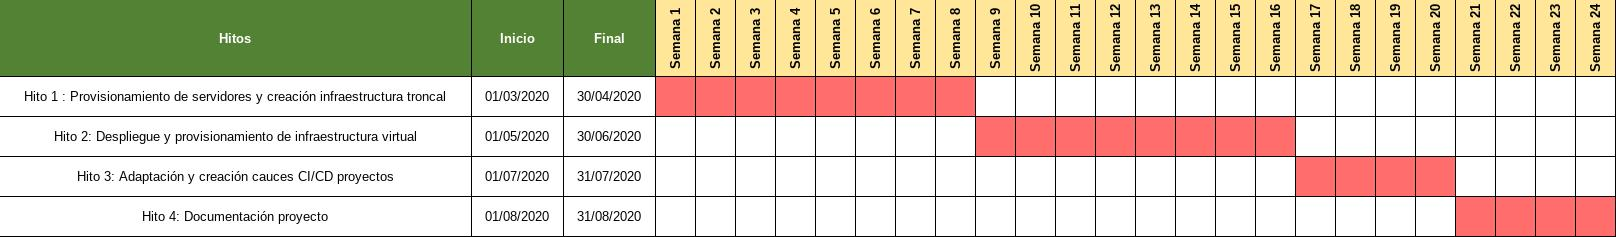
\includegraphics[scale=0.4,angle=-90]{imagenes/Planificacion/gantt.jpg}
		\caption[Diagrama Gantt]{Diagrama Gantt \cite{Gantt:online}} 
		\label{Diagrama Gannt}
	\end{figure}
\clearpage
\section{Presupuesto}
	\begin{text}
		Para realizar este presupuesto, se ha partido del sueldo base de un graduado en Ingeniería Informática. Recalcar que en esta partida, se incluyen horas extra para formación en las tecnologías elegidas.
		Por otra parte se ha incluido en el presupuesto el coste de mantenimiento de la infraestructura.
	\end{text}
	\\
	\begin{table}[ht]
		\centering
		\begin{tabular}[!hbt]{SSSSSSSS} \toprule
			{Concepto} &  {Precio / mes \euro} & {Importe Total \euro} \\ \midrule
			{\textbf{Partida Personal}} \\ \midrule
			{Sueldo DevOps Junior}  & {1.800} & {10.800}  \\
		    \midrule
			{\textbf{Partida Inventariable}} \\ \midrule
			{Coste infraestructura}  & {61,34}  & {368,04}   \\
			\midrule
			{\textbf{Partida Fungible}} \\ \midrule
			{-}  & {-}  & {-}   \\
			\midrule
			{\textbf{Partida servicios técnicos}} \\ \midrule
			{Mantenimiento}  & {Incluido}  & {0} \\
			\midrule	
			{\textbf{Partida viajes y dietas}} \\ \midrule
			{-}  & {-}  & {-} \\
			\midrule	
			{\textbf{Partida de otros}} \\ \midrule
			{Incluido}  & {Incluido}  & {0} \\
			\midrule	
			{\textbf{Total}}  & {1861,34}  & {11.168,04} \\
			\\ \midrule
		 \\ \bottomrule
		\end{tabular}
		\caption[Presupuesto]{Presupuesto \cite{presupuesto:online}} 
		\label{Presupuesto}
	\end{table}

	\begin{text}
		Cabe destacar que en esta partida únicamente se incluyen el coste de un empleado Junior y el coste de la infraestructura necesaria para desarrollar este proyecto. Nótese que en ningún caso, se están añadiendo costes de oficina ni de equipo para desarrollo. En una partida real, habría que incluir estos gastos ya que son imprescindibles para el proceso de desarrollo. En este presupuesto aparece como Otros.
	\end{text}